\newpage
\section{Исследование и построение решения задачи}
\label{research}
% В разделе «Исследование и построение решения задачи» должна быть проведена
% декомпозиция исходной задачи на последовательность подзадач, которые нужно
% решить для получения решения исходной задачи, приведены обосновании всех
% принимаемых решений. Например, если принимается решение о создании некоторого
% программного средства, то необходимо показать, что не существует средства,
% обладающего нужными характеристиками. Исключение составляет случай, когда
% такое средство создается в учебных целях. Обоснование может быть дано одним
% из следующих способов:
% 1.Экспертный: приводятся высказывания, мнения авторитетных специалистов, с
% указанием ссылок на источники, где оно сформулировано;
% 2.Дедуктивный: яркий пример математика - есть система аксиом и правил вывода.
% Если ты сумел показать, как вывести свое утверждение из аксиом с помощью
% правил вывода, то все обосновано.
% 3.Естественнонаучный: выдвигается
% гипотеза (то, что обосновываем) и проводится серия экспериментов, на основании
% обработки результатов этих экспериментов гипотеза либо подтверждается, либо нет
% 4. Инженерно-практический:  хорош когда в качестве утверждения выступает некий
% принцип или система, работоспособность которого мы хотим обосновать, тогда
% экспериментальная реализация может выступать в качестве обоснования..

Для того, чтобы применить метод опорных векторов к задаче фильтрации спама,
необходимо научиться представлять письма в виде, пригодом для применения
этого метода - в виде вектора признаков.
Кроме того нам необходимо построить многопрофильную систему, а для этого
классифицируемый вектор должен содержать какую-то информацию о пользователе.

\subsection{Выделение лексем}
Под \textbf{лексемами} мы будем понимать последовательности символов, на которые мы разбиваем исходный текст. В некотором смысле лексема - это аналог слова. Выделить слова из текста зачастую бывает затруднительно, кроме того зачастую смысловую нагрузку несет лишь часть слова, а иногда напротив лишь последовательность слов. Для разбиения текста на лексемы существует несколько способов:
\begin{itemize}
\item \textbf{Разбиение до пробельных символов или знаков препинания}. В этом случае лексема получается практически полным аналогом слова. Например текст ``Как хорошо, замечательно жить в этом мире!'' разобьется на следующие лексемы:
 ``Как'' , ``хорошо'', ``замечательно'', ``жить'', ``в'', ``этом'' и ``мире''.

 \item \textbf{Выделенеие n-грамм}. В этом случае из текста выделяются все цепочки содержащие ровно n символов. Например при n=6 фраза ``hello, world'' породит следующие 6-граммы: ``hello,'', ``ello, '', ``llo, w'', ``lo, wo'', ``o, wor'', ``, worl'' и `` world''.

 \item \textbf{Выделение цепочек}. Использование в качестве лексем цепочек из нескольких слов. При этом в качестве лексем выделяются как сами слова, так и последовательности из нескольких подряд идущих слов. Например ``free viagra'' породит лексемы ``free'', ``viagra'' и ``free viagra''.
\item {Выделение частичных цепочек}. Этот алгоритм рассматривает окна из нескольких слов, и генерирует цеочки состоящие из некоторых(необязательно идущих подряд) слов этого окна. Например, из  текста ``the quick brown fox jumped'' при размере окна 4 будут сгенерированы такие, как ``the quick brown *'', ``quick * * jumped'', ``* * * jumped'' и другие.

\item {Выделение биграмм}. Алгоритм похож на использование частичных цепочек, однако генерирует только те цепочки, в которых содержится ровно два слова. Для предыдущего примера алгоритм сгенерирует цепочки ``the quick * *'' ``* * brown jumped'', ``the * * fox''  и другие.
\end{itemize}

В dspam можно по желанию использовать любой из алгоритмов, но по умолчанию используется метод выделения цепочек. Разработчики dspam указывают\cite{TOKS} что применительно к задаче фильтрации спама такой метод работает не хуже других. Для решения нашей задачи мы также воспользуемся этим методом.

Так как термин \textbf{лексема} по смыслу близок к слову в обычном понимании, то в дальнейшем говоря о частотах слов мы будем подразумевать частоты лексем.

\subsection{Представление письма в векторном виде}
\label{MESSAGEVECTOR}
Метод опорных векторов работает с объектами, представленными в векторном виде.
Письма имеют текстовую, структуру. Однако у электронного сообщения возможно выделить большое количество
числовых признаков, например:
\begin{itemize}
    \item Количество слов в письме;
    \item Дата отправления;
    \item Количество заголовков;
    \item Количество вложений.
\end{itemize}
Все эти признаки в принципе могут быть использованы для построения векторного
представления письма, однако они никак не передают самое важное, что отличает
спам от легитимной почты - смысл сообщения.

\begin{figure}[h]
\begin{center}
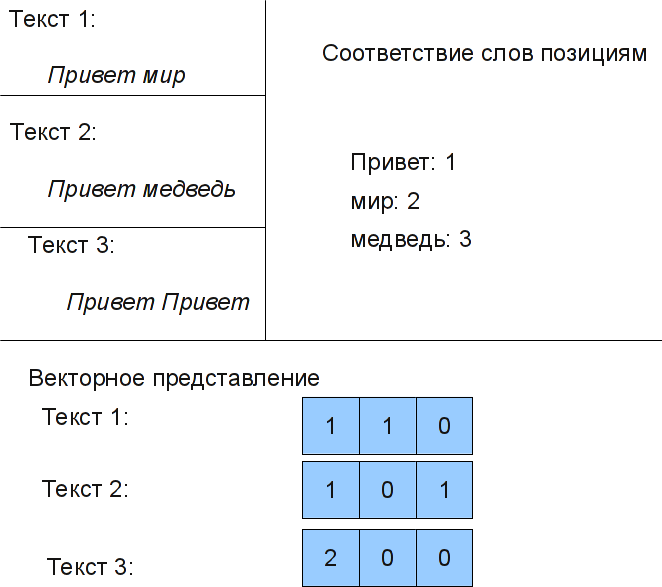
\includegraphics[width=10cm]{img/vectorize}
\end{center}
\caption{Векторное представление текста}
\label{svm-kernel}
\end{figure}

Человек, для того, чтобы понять смысл текста, анализирует совокупность слов в этом тексте.  Хорошей характеристикой тематики текста являются частоты входящих в него слов.
Таким образом мы можем взять все слова в языке, посчитать количество каждого из них в письме
и получить вектор частот.

Проблема заключается в том, что размерность такого вектора черезмерно высока, причем
почти все признаки в этом случае окажутся нулевыми. Русский язык содержит около 100000 слов, а с
учетом словоформ количество слов может превысить несколько миллион.

Скорость работы метода опорных векторов линейно зависит размерности пространства классифицируемых векторов.
Большая размерность вектора приведет к увеличению времени построения модели и времени классификации.
Кроме того метод склонен к переобучению при больших размерностях векторов. Поэтому необходимо каким-то образом ограничить количество используемых для классификации слов.

Для решения задачи выбора используемых для классификации была произведена серия экспериментов.
Были протестированы следующие способы отбора:
\begin{itemize}
\item Выбор наиболее частых слов
\item Выбор случайно отобранных слов
\item Выбор слов для которых разница между частотой появления в спаме и в легитимной почте максимальна
\end{itemize}

Экспериментальным путем было установленно что наилучшие результаты метод опорных векторов проявляет при использовании 1500 самых частых слов. При меньшем количестве информации слишком мало для классификации, при большем - начинают проявляться проблемы переобучения.

\subsection{Многопрофильность}
По постановке задачи необходимо построить такой классификатор, который должен сочетать достоинства персонифицированного и неперсонифицированного подходов. 

Таким образом при классификации письма должна учитываться информация о конкретном адресате. Получается что классификатор должен представлять из себя не просто функцию $F(M)$, где $M$ - сообщение, а функцию $F(A, M)$ - где $A$ - информация об адресате письма. 
Обучающая выборка в таком случае будет состоять из троек $(A, M, S)$  где $A$ и $M$ - информация о пользователе и сообщение, а $S$ - принадлежность письма к конкретному классу.

В качестве такой информации удобно взять идентификатор пользователя в почтовой системе. Любая другая информация может быть восстановлена из обучающей выборки, а значит будет заведомо излишней.

Для применения метода опорных векторов необходимо уметь представлять пару $(A, M)$ в виде вектора. Для этого достаточно представлять в виде вектора. Для этого достаточно представить в виде вектора $A$ и $M$, а потом выполнить конкатенацию этих векторов.

Как представить в виде вектора $М$ было показано в разделе \ref{MESSAGEVECTOR}. Выше было показано, что $A$ можно представить в виде одного числа - id пользователя в почтовой системе. Таким образом мы можем всю пару представить в виде вектора, в котором на первой позиции стоит id пользователя, а дальше векторное представление письма. 

Id пользователя является номинальным признаком(признаком который может принимать лишь конечное количество значений), однако методы машинного обучения(и в частности SVM\cite{YURYSVM}) не очень хорошо ведут себя в случае номинальных признаков.
Для решения проблемы используется ``бинаризация'' признаков - один номинальный признак, принимающий значения от 1 до $N$ заменяется $N$ бинарными признаками $\phi_1 ... \phi_N$. 

При этом $\phi_i$ принимает значение 1 тогда и только тогда, когда исходный признак равен $i$, в противном случае $\phi_i$ принимает значение 0.

Покажем, что при таком представлении пар (пользователь, письмо) действительно будут совмещаться достоинтства персонифицированного неперсонифицированного подходов. 

Рассмотрим ситуацию, когда в системе существует пользователь, который еще не добавлял своих писем в обучающую выборку. В таком случае при работе метода опорных векторов такое письмо попадет в спам тогда, когда у большей части пользователей оно бы склассифицировалось как спам. Таким образом проблема нового пользователя будет решена - даже без предварительной настройки пользователь получает работающую систему фильтрации спама.

В ситуации когда пользователь уже добавлял письма похожего типа в свою обучающую выборку наиболее близким к вновь пришедшему письму будет письмо, которое было у данного пользователя. Таким образом письмо склассифицируется с учетом специфики данного конкретного пользователя.

Таким образом общая схема получения вектора из письма такова:
\begin{itemize}
	\item Строится вектор частот.
	\item Строится вектор, идентицирующий пользователя.
	\item Два вектора конкатенируются, получается результирующий вектор.
\end{itemize}

\begin{figure}[h]
\begin{center}
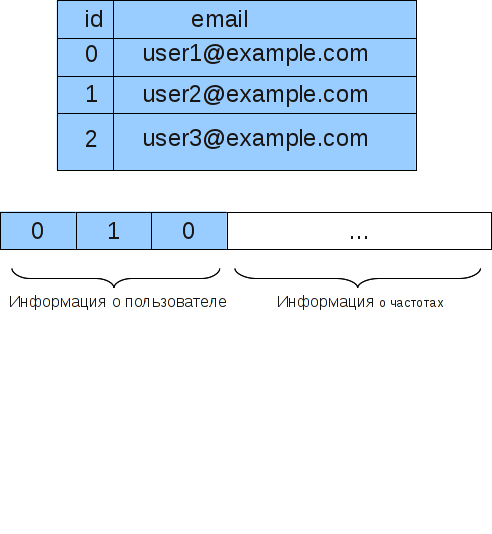
\includegraphics[width=10cm]{img/add_uid}
\end{center}
\caption{Добавление информации о профиле в вектор письма. Письмо адресовано второму пользователю.}
\label{multiprofile}
\end{figure}

